\documentclass[11pt]{article}
\usepackage[a4paper,margin=1in]{geometry}
\usepackage{amsmath,amssymb,amsthm,bm}
\usepackage{graphicx}
\usepackage{hyperref}

\usepackage{pgfplots}
\pgfplotsset{compat=1.18}

\title{\textit{\textbf{Technical Report}}\\Chi-squared Cox Processes}
\author{Tilman, Charlotte (?), Adrian (?), others (?), ...}
\date{\today}

\begin{document}
	\maketitle
	
	\section{Introduction}
	Cox processes (doubly stochastic Poisson processes) are a flexible class of models for clustered spatial point patterns. The \emph{log-Gaussian Cox process} (LGCP) is by far the most widely studied and applied, owing to its tractability and natural connection to Gaussian random fields (GRFs). 
	
	An alternative---rarely used in practice---is the \emph{chi-squared Cox process} (CSCP), in which the random intensity is given by the sum of squared Gaussian fields. Despite their similarities, the two processes induce different distributional and clustering properties. This document summarizes key properties of both models, and sketches possible avenues for publication that highlight the merits and potential uses of CSCPs.
	
	\section{Definitions}
	
	\subsection{Log-Gaussian Cox Process (LGCP)}
	An LGCP is defined by
	\[
	\Lambda(s) = \exp\{ Z(s) \}, \qquad s \in D \subset \mathbb{R}^d,
	\]
	where $Z(s)$ is a Gaussian random field with mean function $\mu(s)$ and covariance $C(s,s')$. Conditional on $\Lambda$, the point process $X$ is Poisson with intensity function $\Lambda(s)$.
	
	Key properties:
	\begin{itemize}
		\item $\mathbb{E}[\Lambda(s)] = \exp(\mu(s) + \tfrac{1}{2}\sigma^2)$.
		\item The pair correlation function is
		\[
		g(s,s') = \exp\{ C(s,s') \},
		\]
		showing that clustering strength depends exponentially on covariance. In particular, $g(0)=\exp(\sigma^2)$ can be arbitrarily large.
		\item Widely used in practice: tractable through moment properties, simulation methods, and fitting algorithms (composite likelihood, Bayesian inference, INLA).
	\end{itemize}
	
	\subsection{Chi-squared Cox Process (CSCP)}
	A CSCP is defined by
	\[
	\Lambda(s) = \sum_{i=1}^k Z_i^2(s), \qquad s \in D,
	\]
	where $\{Z_i(s)\}_{i=1}^k$ are independent Gaussian random fields with mean $\mu_i(s)$ and covariance functions $C_i(s,s')$.
	
	Key properties:
	\begin{itemize}
		\item $\mathbb{E}[\Lambda(s)] = \sum_{i=1}^k \big( \mu_i(s)^2 + \sigma_i^2 \big)$.
		\item $\mathrm{Var}[\Lambda(s)] = 2\sum_{i=1}^k \big(\sigma_i^4 + 2\mu_i^2\sigma_i^2 \big)$.
		\item The pair correlation has the form
		\[
		g(s,s') = 1 + \frac{\sum_{i=1}^k \big( \mathrm{Cov}(Z_i(s),Z_i(s')) \big)^2}{\big( \sum_{i=1}^k \sigma_i^2 + \mu_i^2 \big)^2}.
		\]
		In the symmetric zero-mean case, $g(0)=1+2/k$, so clustering strength at very short lags is bounded.
		\item Marginally, $\Lambda(s)$ follows a noncentral chi-squared distribution with $k$ degrees of freedom and noncentrality parameters $\mu_i^2/\sigma_i^2$. These marginals have lighter (exponential) tails compared to the lognormal marginals of an LGCP.
	\end{itemize}
	
	\section{Similarities and Differences}
	
	\subsection*{Similarities}
	\begin{itemize}
		\item Both are Cox processes driven by latent Gaussian random fields.
		\item Both induce clustering via spatial correlation in the latent fields.
		\item Both can represent multi-scale clustering when multiple latent fields with different correlation lengths are included.
		\item Both are second-order intensity reweighted stationary under suitable conditions, allowing use of summary statistics such as the pair correlation function.
	\end{itemize}
	
	\subsection*{Differences}
	\begin{itemize}
		\item \textbf{Marginals:} LGCP intensities are lognormal with heavy tails; CSCP intensities are chi-squared/gamma-like with lighter exponential tails.
		\item \textbf{Pair correlation:} For LGCP, $g(s,s') = \exp\{ C(s,s') \}$ and $g(0)$ can be arbitrarily large; for CSCP, $g(s,s')$ depends quadratically on covariance and $g(0)$ is bounded, yielding less explosive but potentially more interpretable clustering strength.
		\item \textbf{Role of $k$:} The degrees of freedom $k$ in CSCP controls variability and relative clustering. For large $k$, the CSCP intensity approaches Gaussianity by the central limit theorem, reducing to near-homogeneous Poisson behavior.
		\item \textbf{Interpretability:} In LGCP, the log-scale linear predictor is directly interpretable. In CSCP, $k$ may be viewed as the number of independent clustering mechanisms.
	\end{itemize}
	
%	\section{Illustration: Pair Correlation Functions}
	
%	To visualise the contrast, Figure~\ref{fig:gcomp} sketches the typical shapes of 
%	the pair correlation functions $g(h)$ for an LGCP and for a CSCP with two components. 
%	For the LGCP, $g(h)=\exp\{\sigma^2 \rho(h)\}$ grows exponentially with the covariance, 
%	so $g(0)=\exp(\sigma^2)$ can be arbitrarily large. For the CSCP, 
%	$g(h)=1+\frac{\sum_i \sigma_i^4 \rho_i(h)^2}{(\sum_i \sigma_i^2)^2}$, so $g(0)$ is 
%	bounded (e.g.\ $1+2/k$ in the symmetric case), and the shape is additive across scales.
%	

See Figure \ref{fig:basic} for six realisations of a zero-mean, exponential-covariance CSCP with $k=2$.

\begin{figure}
	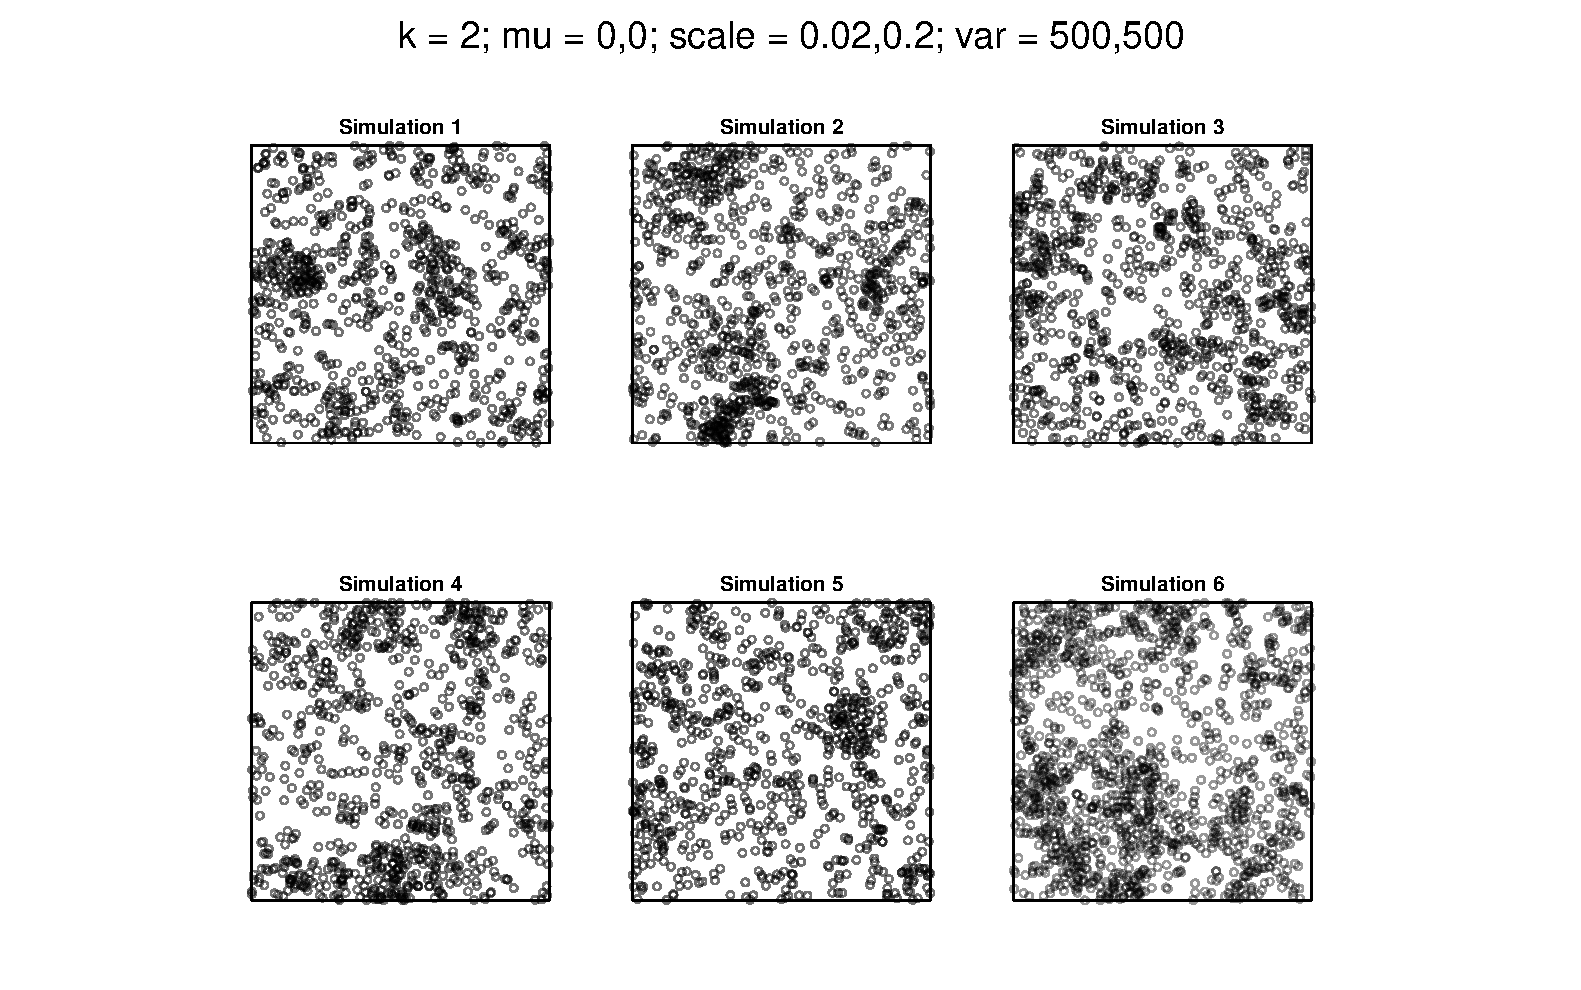
\includegraphics[width=1\textwidth]{fig_basic.pdf}
	\caption{Six replicates of a 2-component CSCP.}\label{fig:basic}
\end{figure}

\section{Covariance structure of the CSCP intensity field}

Let the chi-squared Cox process (CSCP) be driven by $k$ independent Gaussian random fields 
\[
Z_i(s) \sim \mathrm{GRF}\!\big(\mu_i,\, \sigma_i^2 \rho_i(\|s-s'\|)\big), 
\qquad i=1,\dots,k,
\]
where $\mu_i$ is the mean, $\sigma_i^2$ the marginal variance, and 
$\rho_i(h)$ the correlation function at spatial lag $h=\|s-s'\|$. 
The random intensity is
\[
\Lambda(s) = \sum_{i=1}^k Z_i(s)^2 .
\]

\subsection{Mean intensity}
By independence across $i$,
\[
\mathbb{E}\{\Lambda(s)\}
= \sum_{i=1}^k \mathbb{E}\{Z_i(s)^2\}
= \sum_{i=1}^k \big(\mu_i^2 + \sigma_i^2\big).
\]

\subsection{Covariance function (general case)}
For any two locations $s,s'$ with separation $h=\|s-s'\|$,
\[
\operatorname{Cov}_\Lambda(h) 
= \operatorname{Cov}\!\big(\Lambda(s), \Lambda(s')\big)
= \sum_{i=1}^k \operatorname{Cov}\!\big(Z_i(s)^2, Z_i(s')^2\big),
\]
since the fields are independent across $i$.

Applying Isserlis’ (Wick’s) theorem for fourth moments of Gaussians,
\[
\mathbb{E}[Z_i(s)^2 Z_i(s')^2]
= \mathbb{E}[Z_i(s)^2]\,\mathbb{E}[Z_i(s')^2]
+ 2\,\big(\operatorname{Cov}(Z_i(s),Z_i(s'))\big)^2.
\]

Thus
\[
\operatorname{Cov}\!\big(Z_i(s)^2,Z_i(s')^2\big)
= 2 \big(\sigma_i^2 \rho_i(h)\big)^2 \;+\; 4 \mu_i^2 \sigma_i^2 \rho_i(h).
\]

Hence the full covariance is
\[
\boxed{\;
	\operatorname{Cov}_\Lambda(h) 
	= \sum_{i=1}^k \Big[\,2 \sigma_i^4 \rho_i(h)^2 \;+\; 4 \mu_i^2 \sigma_i^2 \rho_i(h)\,\Big].
	\;}
\]

\subsection{Zero-mean special case}
If $\mu_i=0$ for all $i$, this reduces to
\[
\boxed{\;\;
	\operatorname{Cov}_\Lambda(h) = 2 \sum_{i=1}^k \sigma_i^4 \rho_i(h)^2 .
	\;\;}
\]
This case is often taken as the baseline in the literature (e.g. Møller and Waagepetersen, 2004 \cite{MW2003book}).

\subsection{Pair correlation function}
The pair correlation function is defined as
\[
g(h) \;=\; 1 + \frac{\operatorname{Cov}_\Lambda(h)}{ \big(\mathbb{E}\{\Lambda(s)\}\big)^2 }.
\]
For the zero-mean, equal-variance case with exponential correlation $\rho_i(h) = \exp(-h/\phi_i)$, 
\[
g(h)-1 \;=\; \sum_{i=1}^k b_i \, e^{-2h/\phi_i},
\qquad 
b_i = \frac{2\sigma_i^4}{\Big(\sum_{j=1}^k \sigma_j^2\Big)^2}.
\]

\subsection{Semilog transformation and scale identification}
Writing $y(h)=g(h)-1$, for two components we have
\[
y(h) = b_S e^{-2h/\phi_S} + b_L e^{-2h/\phi_L}.
\]
Taking logs,
\[
\log y(h) = \log b_S - \tfrac{2h}{\phi_S} 
+ \log\!\left(1 + \tfrac{b_L}{b_S} e^{-2h\left(\tfrac{1}{\phi_L}-\tfrac{1}{\phi_S}\right)}\right).
\]

This is a log-sum-exp form: globally curved, but in limiting regimes it becomes linear:
\begin{align*}
	\log y(h) &\approx \log b_S - \tfrac{2h}{\phi_S}, && \text{if small scale dominates},\\
	\log y(h) &\approx \log b_L - \tfrac{2h}{\phi_L}, && \text{if large scale dominates}.
\end{align*}
The crossover (“shoulder”) occurs at 
\[
h^\star = \frac{\phi_S \phi_L}{2(\phi_L - \phi_S)} 
\log\!\Big(\tfrac{b_S}{b_L}\Big).
\]

Thus, on a semilog plot of $g(h)-1$, the CSCP naturally reveals its modular structure: 
straight-line regimes with slopes $-2/\phi_S$ and $-2/\phi_L$, with the transition at $h^\star$. See Figure \ref{fig:csclgcp-semilog}.


\begin{figure}[h]
	\centering
	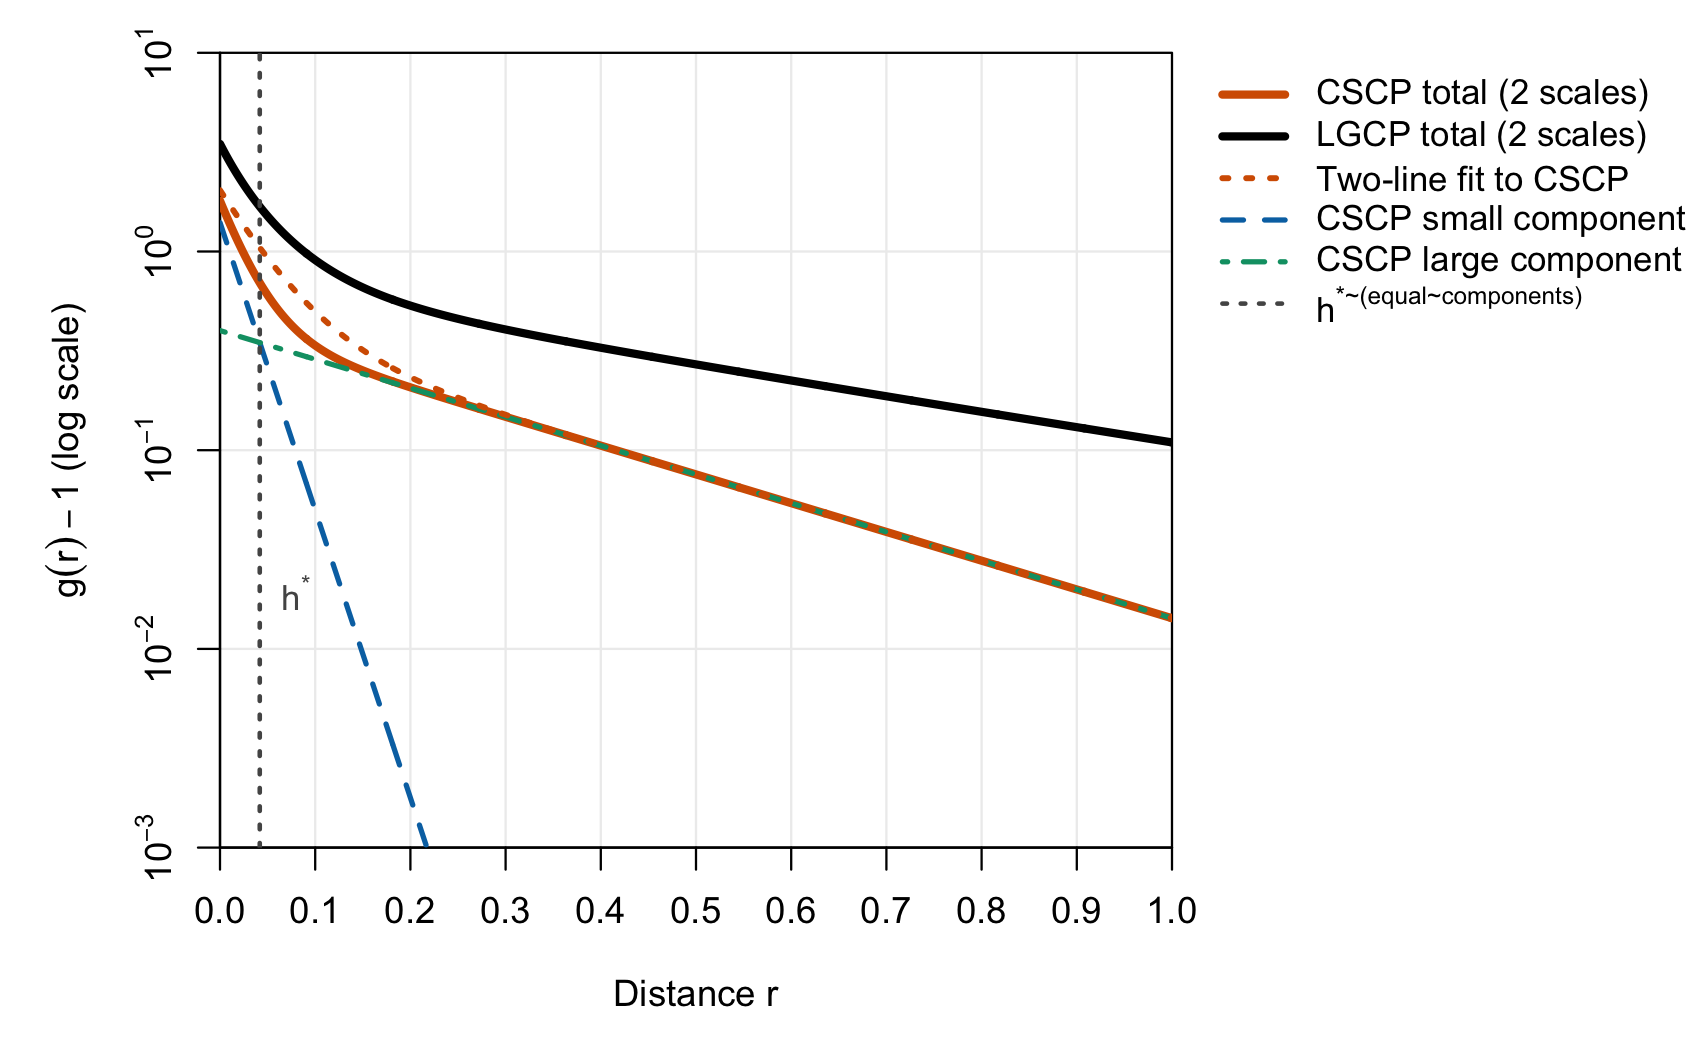
\includegraphics[width=1\textwidth]{semilog_gminus1_with_LGCP.png}
	\caption{Semilogarithmic plot of $g(h)-1$ for a two-scale CSCP. 
		Because $g(h)-1 = b_S e^{-2h/\phi_S} + b_L e^{-2h/\phi_L}$, the function is a sum of exponentials. 
		On the semilog scale, this produces two approximately linear regimes: one at small lags with slope $-2/\phi_S$ (short-range clustering), 
		and one at larger lags with slope $-2/\phi_L$ (long-range clustering). 
		The vertical marker denotes the crossover distance $h^\star$, where the two component contributions are equal. 
		This ``shoulder'' provides a natural diagnostic of the modular structure of CSCPs, 
		in contrast to LGCPs where multiple scales are entangled in the exponent and the curve remains smoothly curved.}
	\label{fig:csclgcp-semilog}
\end{figure}



\paragraph{Reconstruction by two-line regression.}
In Figure \ref{fig:csclgcp-semilog}, the orange dotted line is an {estimate} of $g(h)-1$ obtained by a simple two-line procedure:
\begin{enumerate}
	\item Select two ranges of $h$: one where the short-scale term dominates, another where the long-scale term dominates.
	\item On each range, regress $\log\{g(h)-1\}$ on $h$ to obtain a slope $m$ and intercept $c$.
	\item Translate these line parameters back into exponential form:
	\[
	\widehat{\phi} = -\tfrac{2}{m}, \qquad \widehat{b} = e^c.
	\]
	\item Combine the two estimated exponentials:
	\[
	\widehat{y}(h) \;=\; \widehat{b}_S e^{-2h/\widehat{\phi}_S} 
	+ \widehat{b}_L e^{-2h/\widehat{\phi}_L}.
	\]
\end{enumerate}

This is capable of reproducing the true CSCP curve closely when the two scales are well separated. The key diagnostic feature is that the CSCP decomposes naturally into additive straight lines on the log scale, making its modular structure identifiable. In contrast, the LGCP curve (black) remains smoothly curved on this scale and does not admit such a decomposition.

\section{Comparison: LGCP pair correlation}

For a two-scale log-Gaussian Cox process (LGCP), the pair correlation is
\[
g(h) \;=\; \exp\!\Big\{ C_S(h) + C_L(h) \Big\},
\]
where $C_S(h), C_L(h)$ are the covariance functions of the short- and long-range Gaussian fields (e.g.\ exponential or Matérn).  

\paragraph{Log structure.}
Unlike the CSCP, taking logarithms does not linearise $g(h)-1$:
\[
\log\!\big( g(h)-1 \big) \;\approx\; C_S(h) + C_L(h),
\]
which is the \emph{sum of covariance functions}, not a sum of exponentials.  
On a semilog plot of $g(h)-1$, the curve remains smoothly curved — there are no clean straight-line regimes.

\paragraph{No modular decomposition.}
For the LGCP, the short- and long-scale contributions enter additively \emph{inside the exponent}, so their effects are inseparably entangled. This produces a global smoothness: there is no finite interval of $h$ where one scale contributes a straight line independent of the other.

\paragraph{Contrast with CSCP.}
The LGCP curve (black in Figure \ref{fig:csclgcp-semilog}) bends continuously, while the CSCP curve (orange) is well approximated by the sum of two linear regimes on the semilog scale.  
This is the key diagnostic difference:
\begin{itemize}
	\item \textbf{CSCP}: additive structure in $g(h)-1$ itself $\;\to\;$ modular, identifiable scales.
	\item \textbf{LGCP}: additive structure in the exponent $\;\to\;$ smooth entanglement of scales, no modular separation.
\end{itemize}

Thus, while the two models can look superficially similar on a linear scale, the semilog representation reveals that only the CSCP decomposes naturally into interpretable multi-scale contributions.


\section{Dealing with the mean}
We'd like to control the expected number of points, preferably decoupling from the variance(s). A natural first attempt at a stationary reparameterisation is to work with
\[
\bar\lambda, \quad w \in [0,1], \quad \{\alpha_i\}_{i=1}^k, \quad \sum_i \alpha_i = 1,
\]
where $\bar\lambda$ is the target mean intensity, $w$ allocates the proportion of this mean explained by the stochastic CSCP component, and $\alpha_i$ partitions $w\bar\lambda$ across the $k$ Gaussian-field summands.  In this scheme one sets
\[
\sigma_i^2 = w \, \bar\lambda \, \alpha_i, 
\qquad \mu_i = 0,
\]
so that the overall mean is respected.

\paragraph{Limitations.}
This parameterisation has several drawbacks:
\begin{itemize}
	\item \emph{Entanglement of mean and variance:} Since the variances $\sigma_i^2$ are tied directly to $\bar\lambda$, increasing the expected number of points also changes the second-order clustering structure. Thus a dataset with 100 points and one with 10{,}000 points would imply different $g(h)$ curves even if the underlying spatial correlation should be the same.
	\item \emph{Lack of invariance:} For a Cox process one would ideally like the pair correlation $g(h)$ to depend on correlation ranges $\phi_i$ and relative weights $\alpha_i$, not on the overall sample size. The above construction does not preserve this invariance.
	\item \emph{Identifiability issues:} Different combinations of $(\bar\lambda, w, \alpha_i)$ can lead to the same mean intensity but distinct implied clustering, making fitted values hard to interpret. With large $k$ this risks overfitting.
\end{itemize}

\paragraph{Alternative: Mean-invariant scaling.}
A cleaner approach is to decouple the first- and second-order structures. One may write
\[
\Lambda(s) = \lambda_0 + \sum_{i=1}^k Z_i^2(s),
\]
with $\lambda_0$ as a separate baseline mean intensity, and $Z_i$ Gaussian fields with variance parameters $\sigma_i^2$ and ranges $\phi_i$. Here the expected total intensity is governed by $\lambda_0 + \sum_i \sigma_i^2$, while the pair correlation function is determined entirely by $(\sigma_i^2, \phi_i)$. This ensures that increasing $\bar\lambda$ via $\lambda_0$ does not alter the shape of $g(h)$, giving stable second-order behaviour across sample sizes.

\paragraph{Caution on $k$.}
Although the mean-invariant form has cleaner separation, identifiability remains delicate when many components are allowed. With $k\geq 3$ it becomes increasingly difficult to distinguish overlapping scales, and parameter trade-offs between $\lambda_0$ and $\{\sigma_i^2\}$ can emerge. In practice, 2--3 components are likely the most defensible balance between flexibility and identifiability.




\section{Fitting a multi-scale CSCP under mean-stationarity}

For a stationary $k$--component CSCP, suppose we write the intensity  as
\[
\Lambda(s) \;=\; \lambda_0 \;+\; \sum_{i=1}^k Z_i(s)^2,
\qquad
Z_i(s)\sim \text{GRF}\big(0,\;\sigma_i^2 \rho_i(\|h\|)\big),
\]
where $\lambda_0 \ge 0$ is a deterministic baseline, and the $Z_i$ are independent zero-mean Gaussian random fields with marginal variances $\sigma_i^2$ and correlation functions $\rho_i(h)$.  

\subsection{The mean--variance entanglement problem}

If we set $\lambda_0=0$, then
\[
\mathbb E\{\Lambda(s)\} = \sum_{i=1}^k \sigma_i^2,
\]
and the pair correlation takes the form
\[
g(h)-1 = \frac{2\sum_{i=1}^k \sigma_i^4\,\rho_i(h)^2}{\big(\sum_{j=1}^k \sigma_j^2\big)^2}.
\]
As noted above, the same parameters $\sigma_i^2$ simultaneously control both the \emph{first order} (mean intensity) and the \emph{second order} (clustering strength).  
This is undesirable in practice: if the observed pattern has, say, 1000 points, we do not want all of that count to be explained entirely by the $\sigma_i^2$, since their role should be primarily to govern the second-order properties.

\subsection{Trying to decouple the mean from the second order}

Include a non-random baseline $\lambda_0$, and reparameterize as follows. Let $\bar\lambda$ denote the desired stationary mean intensity of the process. Introduce:
\begin{itemize}
	\item a mean fraction $w \in (0,1)$ specifying the ``proportion of $\bar\lambda$ explained by the random components'',
	\item weights $\alpha_i \ge 0$ with $\sum_{i=1}^k \alpha_i = 1$, allocating that random fraction across components,
	\item a baseline $\lambda_0 = (1-w)\bar\lambda$.
\end{itemize}
Then define
\[
\sigma_i^2 = w\,\bar\lambda\,\alpha_i, \qquad i=1,\ldots,k.
\]

By construction,
\[
\mathbb E\{\Lambda(s)\} = \lambda_0 + \sum_i \sigma_i^2 = (1-w)\bar\lambda + w\bar\lambda = \bar\lambda,
\]
so the total mean intensity is decoupled and controlled directly by $\bar\lambda$. But there is still a clear link to $\sigma_i^2$ (see above), so I'm not sure this will work.

\subsection{Pair correlation under this parameterization}

Substituting into the expression for $g(h)-1$, we obtain
\[
g(h)-1 = 2w^2 \sum_{i=1}^k \alpha_i^2 \,\rho_i(h)^2.
\]

This has the following features:
\begin{itemize}
	\item The overall mean $\bar\lambda$ no longer appears in the pair correlation, so estimation of second-order properties is stable and independent of the mean.
	\item The parameter $w$ directly controls the overall clustering strength: $w=0$ gives a homogeneous Poisson process, while larger $w$ increases the variance-to-mean ratio.
	\item The parameters $\alpha_i$ and $\phi_i$ (through $\rho_i$) control the relative contributions and correlation scales of the components.  
\end{itemize}

\subsection{Practical implications}

This reparameterization cleanly separates the roles of the parameters:
\begin{itemize}
	\item $\bar\lambda$: fixes the average number of points (first order).
	\item $w$: governs the overall clustering amplitude.
	\item $\{\alpha_i,\phi_i\}$: control the decomposition of clustering across scales.
\end{itemize}

Thus, the $\sigma_i^2$ need not be “responsible” for the mean. Instead, they inherit values consistent with $(\bar\lambda,w,\alpha_i)$, leaving $\phi_i$ and $\alpha_i$ to shape the second-order structure. This addresses the entanglement problem and (maybe?) provides a principled, interpretable framework for fitting multi-scale CSCPs in practice.

\subsection{Identifiability considerations}

The proposed parameterisation separates the mean intensity $\bar\lambda$, the clustering amplitude $w$, and the component weights $\alpha_i$.  
In practice, their identifiability depends on which order of properties is being used:

\begin{itemize}
	\item \textbf{First order:} The average point count identifies $\bar\lambda$ directly, up to the window size. This is estimable from the data without reference to second-order structure.
	
	\item \textbf{Second order:} The pair correlation function depends only on the \emph{relative} contributions of the random components:
	\[
	g(h)-1 \;=\; 2w^2 \sum_{i=1}^k \alpha_i^2 \rho_i(h)^2.
	\]
	Thus, the $w$ parameter is identifiable only through the \emph{overall amplitude} of clustering, while the $\alpha_i$ are identifiable up to their relative proportions given distinct correlation scales $\phi_i$.
	
	\item \textbf{Interaction of parameters:} $\bar\lambda$ does not appear in $g(h)-1$, so it is cleanly separated. However, $w$ and the $\alpha_i$ always enter together as the combination $w^2 \alpha_i^2$. Hence:
	\begin{itemize}
		\item $w$ is estimable from the global variance-to-mean ratio (how clustered the process is overall),
		\item $\{\alpha_i,\phi_i\}$ are estimable from the \emph{shape} of $g(h)-1$ (multi-scale decay).
	\end{itemize}
\end{itemize}

\paragraph{Practical implication.}
Identifiability is going to be bad in small samples: different $(w,\alpha)$ combinations can mimic each other if the $\phi_i$ are similar.  
But when scales are well separated, the log-representation of $g(h)-1$ should show clear linear regimes, making $w$, $\alpha_i$, and $\phi_i$ practically estimable.  
Thus, the reparameterisation is both interpretable and identifiable, provided that the components act on distinct spatial ranges.

\subsection{Large $k$ is gonna be shithouse, almost surely}

While the CSCP reparameterisation $(\bar\lambda,\; w,\; \{\alpha_i,\phi_i\}_{i=1}^k)$ is interpretable, it's easy to see that identifiability will deteriorate as $k$ grows. The reason is twofold:

\begin{enumerate}
	\item 
	The second-order signal is
	\(
	g(h)-1 \;=\; 2w^2\sum_{i=1}^k \alpha_i^2\,\rho_i(h;\phi_i)^2.
	\)
	If several $\phi_i$ are similar, their contributions are nearly collinear on $\log\{g(h)-1\}$, 
	making $(\alpha_i,\phi_i)$ poorly separated. Finite window size, edge correction, and binning 
	further reduce the `effective resolution' of distinct decay rates.
	
	\item 
	Only the products $w^2\alpha_i^2$ (modulated by $\rho_i^2$) enter $g(h)-1$, 
	so $w$ and $\{\alpha_i\}$ trade off unless the \emph{shape} information (from distinct $\phi_i$) is strong. 
	With larger $k$, different mixtures can fit $g(h)$ nearly equally well.
\end{enumerate}

So, if using this version we should:
\begin{itemize}
	\item \textbf{Prefer small $k$ (e.g.\ $k=2$ or $3$).}
	Choose the smallest $k$ that explains the dominant slope regimes on the semilog plot of $\hat g(h)-1$.
	\item \textbf{Enforce ordering and separation.}
	Constrain $0<\phi_1<\cdots<\phi_k$ and, if needed, a minimal separation 
	(e.g.\ $\phi_{i+1}/\phi_i \ge \delta>1$) to avoid label switching and near-duplicates.
	\item \textbf{Penalise complexity.}
	Use information criteria tailored to second-order/composite fits (e.g.\ CL-AIC/CL-BIC) 
	or cross-validated contrast on $\hat g(h)$ when comparing $k$.
	\item \textbf{Stabilise weights.}
	Parameterise $\alpha_i=\exp(\eta_i)/\sum_j \exp(\eta_j)$ 
	and add a mild ridge penalty on $\eta$ (or a Dirichlet prior in a Bayesian fit) 
	to discourage spurious tiny components.
	\item \textbf{Use robust initialisation.}
	Detect slope plateaus on $\log\{\hat g(h)-1\}$ via sliding-window regressions 
	and change-point segmentation; initialise $(\phi_i,\alpha_i)$ from these plateaus, then refine.
	\item \textbf{Quantify uncertainty.}
	Report bootstrap intervals for $(\phi_i,\alpha_i,w)$ 
	or standard errors from a pairwise/composite likelihood.
	Wide intervals or unstable plateaus will be a red flag for excessive $k$.
\end{itemize}

\paragraph{Rule of thumb:}
We could recommend adopting $k=2$ when a clear ``steep then shallow'' pattern appears; 
consider $k=3$ only if a third, visibly distinct linear regime is sustained over a nontrivial range of $h$. 
Otherwise, additional components are likely unidentifiable and amount to overfitting noise.


\subsection{Dealing with $w=1$}

In the current parameterisation, the random part of the
intensity contributes a fraction $w \in [0,1]$ of the total mean, with the
remaining fraction $(1-w)$ assigned to a homogeneous baseline. The special case
$w=1$ corresponds to a \emph{fully stochastic CSCP} in which \emph{all points}
arise from the Gaussian random fields, with no superimposed baseline Poisson
component.

\paragraph{Definition.}
Let $\bar\lambda$ denote the desired stationary mean intensity, and let
$\alpha_1,\ldots,\alpha_k$ be nonnegative weights summing to one. Then define
\[
\sigma_i^2 = \bar\lambda \,\alpha_i, 
\qquad \mu_i = 0,
\qquad
Z_i(s) \sim \text{GRF}\big(0,\; \sigma_i^2\,\rho_i(\|h\|)\big).
\]
The intensity field is
\[
\Lambda(s) = \sum_{i=1}^k Z_i(s)^2.
\]

\paragraph{First-order behaviour.}
By construction,
\[
\mathbb E\{\Lambda(s)\} = \sum_{i=1}^k \sigma_i^2 = \bar\lambda,
\]
so the expected number of points in a region $W$ is $\bar\lambda |W|$.

\paragraph{Second-order behaviour.}
The pair correlation function is
\[
g(h)-1 \;=\; \frac{2\sum_{i=1}^k \sigma_i^4 \rho_i(h)^2}
{\big(\sum_{j=1}^k \sigma_j^2\big)^2}
\;=\; 2\sum_{i=1}^k \alpha_i^2\,\rho_i(h)^2.
\]
Crucially, the factor $\bar\lambda$ cancels: \emph{the shape and strength of
	clustering depend only on the weights $\alpha_i$ and correlation functions
	$\rho_i$, not on the overall mean intensity}. Thus the pair correlation is
invariant to changes in $\bar\lambda$.

\paragraph{Implications for the number of points.}
The expected count scales linearly with $\bar\lambda$, but the \emph{form} of
$g(h)$ is unchanged. However, as in any Cox process, the variance of the total
count grows faster:
\[
\operatorname{Var}(N) = \bar\lambda|W| + \bar\lambda^2 C_W,
\]
where $C_W=\iint_W c(\|s-t\|)\,ds\,dt$ depends on the kernel $c(h)=2\sum_i
\alpha_i^2\rho_i(h)^2$. Consequently, the index of dispersion,
$\operatorname{Var}(N)/\mathbb E[N]$, increases linearly with $\bar\lambda$.
This reflects the natural property that larger populations exhibit more
realisation-to-realisation variability, even though the spatial clustering
structure is unchanged.

\paragraph{Interpretation.}
The case $w=1$ is especially appealing when the scientific assumption is that
\emph{all observed points arise from clustered structure}, without a
homogeneous background. The parameters then separate cleanly as follows:
\begin{itemize}
	\item $\bar\lambda$ controls the expected number of points,
	\item $\alpha_i$ and $\rho_i$ control the relative contribution and spatial
	range of clustering at each scale.
\end{itemize}

Figure \ref{fig:repam} gives realisations of two 2-component CSCPs, one set with $\bar{\lambda}=100$, the other with $\bar{\lambda}=10000$.

\begin{figure}
	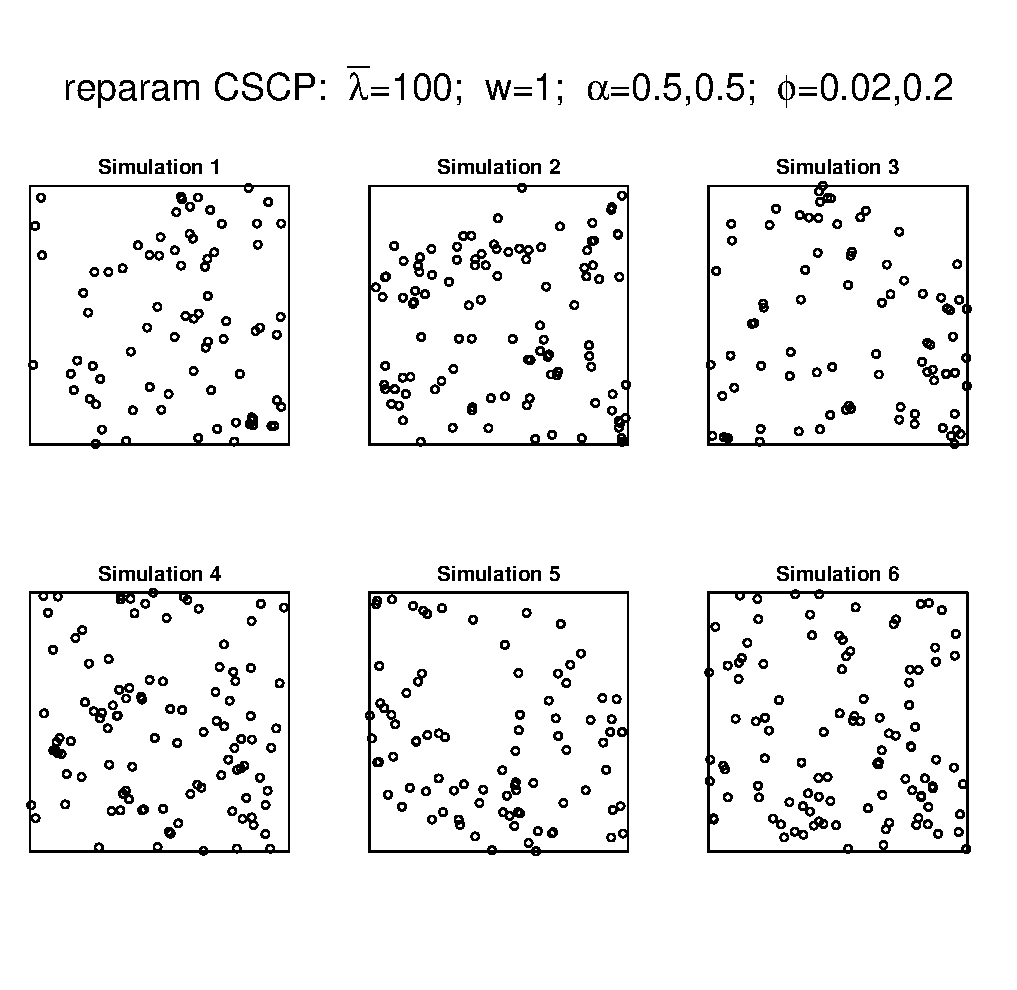
\includegraphics[width=0.7\textwidth]{fig_repam_w1_100.pdf}\\
	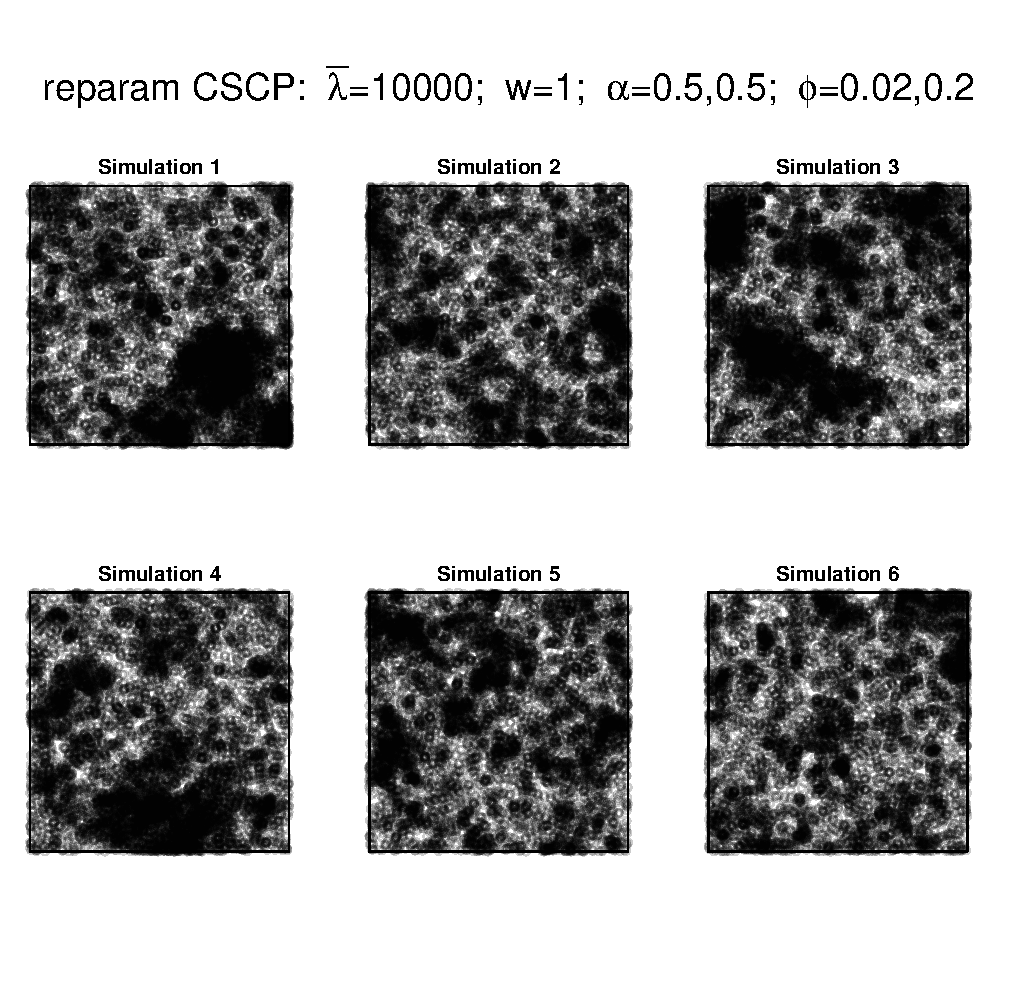
\includegraphics[width=0.7\textwidth]{fig_repam_w1_10000.pdf}\\
	\caption{Two sets of realisations (six each) for $\bar{\lambda}\in\{100,10000\}$, of a reparameterised $k=2$ CSCP with $w=1$ (fully stochastic).}\label{fig:repam}
\end{figure}


\subsection{Dealing with $0<w<1$}

Reminder: $w\in[0,1]$ specifies the fraction of the
mean intensity carried by the \emph{clustered} (random) part, with the remaining
$(1-w)$ assigned to a homogeneous baseline.

\paragraph{Definition.}
Fix a target mean intensity $\bar\lambda>0$ and weights
$\alpha_1,\ldots,\alpha_k\ge 0$ with $\sum_i \alpha_i=1$. Let
\[
\sigma_i^2 \;=\; w\,\bar\lambda\,\alpha_i, 
\qquad \mu_i=0, 
\qquad Z_i(s)\sim \text{GRF}\big(0,\;\sigma_i^2\,\rho_i(\|h\|)\big),
\]
and set the baseline to
\[
\lambda_0 \;=\; (1-w)\,\bar\lambda.
\]
The intensity field is
\[
\Lambda(s) \;=\; \lambda_0 \;+\; \sum_{i=1}^k Z_i(s)^2.
\]

\paragraph{First-order behaviour.}
By construction,
\[
\mathbb E\{\Lambda(s)\}=\lambda_0+\sum_i \sigma_i^2
=(1-w)\bar\lambda+w\bar\lambda=\bar\lambda,
\]
so the expected number of points in a window $W$ is $\bar\lambda\,|W|$.

\paragraph{Second-order behaviour (pair correlation).}
For a Cox process, $g(h)-1=\operatorname{Cov}\{\Lambda(s),\Lambda(t)\}/\mathbb E\Lambda^2$.
Since the baseline is nonrandom, only the squared-field sum contributes to the
covariance. Using independence of the $Z_i$ and Isserlis’ theorem,
\[
g(h)-1 \;=\; 2\,w^2 \sum_{i=1}^k \alpha_i^2\,\rho_i(h)^2.
\]
Hence:
\begin{itemize}
	\item the \emph{shape} across distances is governed by the scales $\rho_i(\cdot)$
	and the composition $\{\alpha_i\}$;
	\item the \emph{amplitude} of clustering is tuned by $w$ (quadratically),
	with $w\!\downarrow\!0$ driving $g(h)\!\to\!1$ (homogeneous Poisson).
\end{itemize}

\paragraph{Implications for the number of points.}
The mean count remains $\mathbb E[N]=\bar\lambda\,|W|$, independently of $w$.
The count variance decomposes as
\[
\operatorname{Var}(N)=\bar\lambda|W| \;+\; (w\,\bar\lambda)^2\,C_W,
\qquad
C_W=\iint_W 2\sum_{i=1}^k \alpha_i^2\,\rho_i(\|s-t\|)^2\,ds\,dt,
\]
so the index of dispersion is
\[
\frac{\operatorname{Var}(N)}{\mathbb E[N]}
\;=\; 1 \;+\; w^2\,\bar\lambda\,\frac{C_W}{|W|}.
\]
Thus, decreasing $w$ damps both small–lag clustering (via $g-1$) and the
between-realisation overdispersion of the total count, while leaving the mean
unchanged.

\paragraph{Interpretation and use.}
The baseline–plus–clustered form is useful when scientific knowledge suggests a
nonzero background of “uninformative” events \emph{in addition} to clustered
mechanisms. Parameters separate cleanly:
\begin{itemize}
	\item $\bar\lambda$ sets the expected number of points (first order);
	\item $w$ controls \emph{how clustered} the pattern is overall (amplitude);
	\item $\{\alpha_i,\rho_i\}$ determine \emph{where and at what scales} clustering
	occurs (shape).
\end{itemize}
As $w\to 1$ we recover the fully stochastic CSCP (no baseline); as $w\to 0$ the
model reduces to a homogeneous Poisson process.

Figure \ref{fig:smallerw} again gives realisations of two 2-component CSCPs, this time with one at $w=0.75$, the other with $w=0.1$ (effectively homogeneous Poisson).

\begin{figure}
	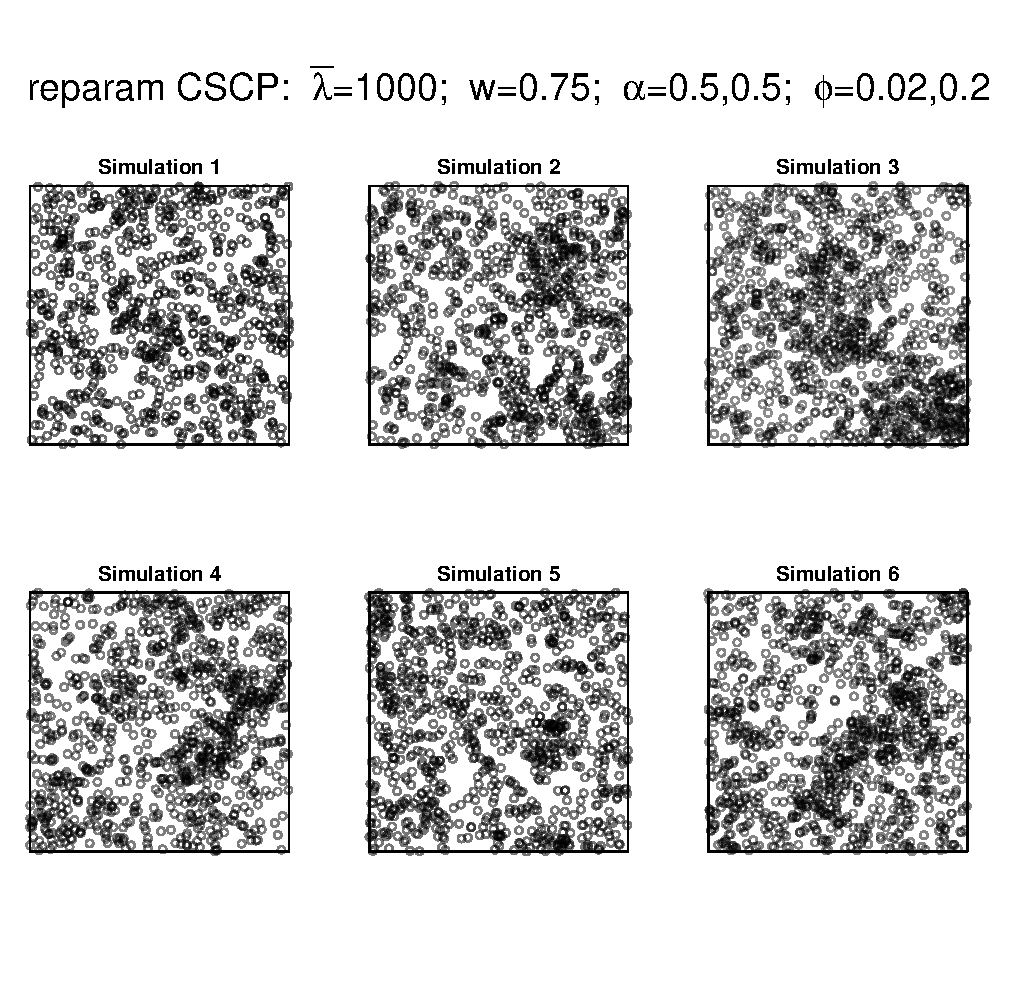
\includegraphics[width=0.7\textwidth]{fig_repam_wsmaller1.pdf}\\
	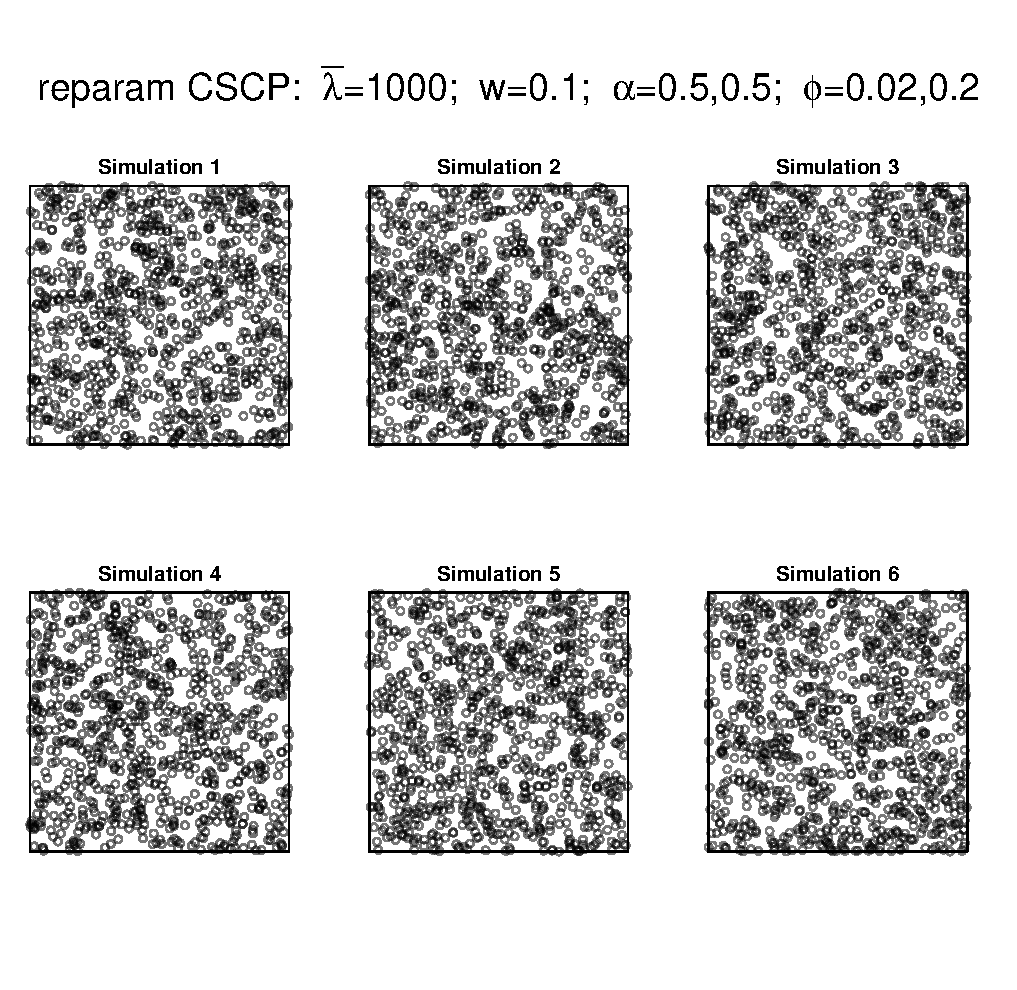
\includegraphics[width=0.7\textwidth]{fig_repam_wsmaller2.pdf}\\
	\caption{Two sets of realisations (six each) for $w\in\{0.75,0.1\}$, of a reparameterised $k=2$ CSCP.}\label{fig:repam}
\end{figure}


\section{Fitting Strategy for CSCPs (\(w=1\))}

We consider the stationary chi-squared Cox process
\[
\Lambda(s) \;=\; \sum_{i=1}^k Z_i(s)^2,
\qquad 
\mathrm{Cov}\{Z_i(s),Z_i(s+h)\} \;=\; \sigma_i^2 \,\rho_i(h;\phi_i),
\]
where the $\{Z_i\}$ are independent, mean-zero Gaussian random fields.  
Define
\[
\alpha_i \;=\; \frac{\sigma_i^2}{\sum_j\sigma_j^2}, \quad 
\sum_i \alpha_i = 1, 
\qquad 
\bar\lambda \;=\; \mathbb E[\Lambda] = \sum_i \sigma_i^2 \;\approx\; \frac{n}{|W|}.
\]

With $w=1$, the pair correlation simplifies to
\[
g(h)-1 \;=\; 2 \sum_{i=1}^k \alpha_i^2 \,\rho(h;\phi_i)^2,
\]
so second-order structure is controlled entirely by $(\alpha,\phi)$, while $\bar\lambda$ fixes the overall scale through $\sigma_i^2 = \bar\lambda \alpha_i$.

\subsection{Case $k=1$: Single-Component CSCP}
When $k=1$, the intensity is $\Lambda(s)=Z(s)^2$ and
\[
g(h)-1 = 2\,\rho(h;\phi)^2.
\]
For an exponential correlation, $\rho(h)=\exp(-h/\phi)$, this reduces to
\[
g(h)-1 = 2\,\exp(-2h/\phi),
\qquad
\log\{g(h)-1\} = \log 2 - \tfrac{2}{\phi}h,
\]
a perfect straight line on semilogarithmic axes.  

\noindent\textbf{Fitting procedure ($k=1$):}
\begin{enumerate}
	\item Compute empirical $\hat g(h)$, set $y(h)=\max\{\hat g(h)-1,\varepsilon\}$.
	\item Fit a linear regression $\log y(h) = c + m h$ over a stable mid-range band $[a,b]$.
	\item Estimate $\hat\phi = -2/m$. The intercept should be close to $\log 2$.
	\item Set $\hat\sigma^2 = \hat{\bar\lambda}$.
	\item Validate using bootstrap envelopes and by checking linearity of $\log\{\hat g(h)-1\}$.
\end{enumerate}

\subsection{Case $k=2$ or $3$: Multi-Component CSCP}
For $k=2$,
\[
g(h)-1 = 2\alpha_1^2 \rho(h;\phi_1)^2 + 2\alpha_2^2 \rho(h;\phi_2)^2,
\]
and similarly for $k=3$. The log--pcf is a \emph{log-sum-exp} of exponentials, producing ``shoulders'' in semilog plots where small-scale and large-scale components trade dominance.

\noindent\textbf{Fitting procedure ($k=2,3$):}
\begin{enumerate}
	\item Compute $\hat g(h)$ and set $y(h)=\max\{\hat g(h)-1,\varepsilon\}$.
	\item On semilog scale, choose disjoint distance bands (small, medium, large).
	\item Fit straight lines $\log y(h) \approx c_i + m_i h$ in each band.
	\item Initialise $\phi_i^{(0)} = -2/m_i$ and $\alpha_i^{(0)} \propto \sqrt{e^{c_i}/2}$ (normalised).
	\item Refine with constrained non-linear least squares (or minimum contrast) enforcing $\alpha_i\ge 0$, $\sum \alpha_i=1$, and ordered scales $\phi_1<\phi_2(<\phi_3)$.
	\item Map back: $\sigma_i^2 = \bar\lambda \alpha_i$.
\end{enumerate}

\subsection{Uncertainty and Diagnostics}
\begin{itemize}
	\item \textbf{Uncertainty:} Use block or toroidal bootstrap, or pairwise composite likelihood with Godambe information.
	\item \textbf{Diagnostics:} 
	\begin{itemize}
		\item For $k=1$, $\log\{g(h)-1\}$ should be nearly linear.
		\item For $k=2,3$, look for piecewise linear regimes on the semilog plot.  
		\item Simulated envelopes for $g$, $K$, and $J$ provide further checks.
	\end{itemize}
\end{itemize}

\subsection{Practical Notes}
\begin{itemize}
	\item $k=1$ serves as a natural baseline; higher $k$ allows modular separation of scales.  
	\item Identifiability improves if $\phi_i$ are well separated.  
	\item Small $k$ (2--3) is defensible; larger $k$ risks overfitting and instability.
\end{itemize}

\begin{quote}
	\noindent\textbf{Intuition: Why semilog regression works for CSCPs.}
	
	\begin{itemize}
		\item \emph{Case $k=1$:}  
		The pair correlation reduces to
		\[
		g(h)-1 \;=\; 2\,e^{-2h/\phi},
		\]
		which is exactly an exponential decay. On semilog axes, $\log\{g(h)-1\}$ is a straight line with slope $-2/\phi$.  
		\textit{Interpretation:} A single scale of clustering produces a single straight line.
		
		\item \emph{Case $k=2$:}  
		Now
		\[
		g(h)-1 \;=\; 2\alpha_1^2 e^{-2h/\phi_1} \;+\; 2\alpha_2^2 e^{-2h/\phi_2},
		\]
		a \emph{sum of two exponentials}. On semilog axes this becomes a log-sum-exp curve: linear at small $h$ (dominated by the short range), linear again at large $h$ (dominated by the long range), with a visible ``shoulder'' where the two contributions cross over.  
		\textit{Interpretation:} Two scales of clustering appear as two approximately straight lines joined by a bend.
	\end{itemize}
	
	\medskip
	\noindent\textbf{Schematic illustration (with guide-lines):}
	
	\begin{center}
		\begin{tikzpicture}[scale=1.1]
			% Axes
			\draw[->] (0,0) -- (3.6,0) node[right] {$h$};
			\draw[->] (0,0) -- (0,2.2) node[above] {$\log\{g(h)-1\}$};
			
			% k=1 straight line
			\draw[thick,blue] (0,1.8) -- (3.2,0.4);
			\node[blue] at (2.65,1.55) {$k=1$};
		\end{tikzpicture}
		\hspace{1.5cm}
		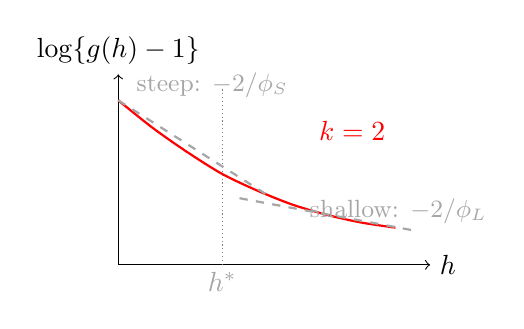
\begin{tikzpicture}[scale=1.1]
			% Axes
			\draw[->] (0,0) -- (3.6,0) node[right] {$h$};
			\draw[->] (0,0) -- (0,2.2) node[above] {$\log\{g(h)-1\}$};
			
			% k=2 shoulder curve (chosen to allow good local tangents)
			\draw[thick,red,smooth] plot coordinates {
				(0.00,1.90) (0.40,1.58) (0.80,1.30) (1.20,1.05)
				(1.60,0.86) (2.00,0.70) (2.40,0.58) (2.80,0.49) (3.20,0.43)
			};
			\node[red] at (2.7,1.55) {$k=2$};
			
			% Shoulder marker (equal-contribution, roughly near h=1.2)
			\draw[densely dotted,gray] (1.20,0) -- (1.20,2.05);
			\node[gray!70] at (1.20,-0.2) {$h^\ast$};
			
			% Dashed guide-lines: choose points so they are visually tangent
			
			% Small-scale (steep) tangent near the left (fits first two curve points)
			% Line through (0.00,1.90) and (0.80,1.30)
			\draw[dashed,gray!70,thick] (0.00,1.90) -- (1.70,0.82);
			\node[gray!70,anchor=south west] at (0.10,1.82) {\small steep: $-2/\phi_S$};
			
			% Large-scale (shallow) tangent on the right (fits two rightmost curve points)
			% Line through (2.40,0.58) and (3.20,0.43)
			\draw[dashed,gray!70,thick] (1.40,0.77) -- (3.40,0.40);
			\node[gray!70,anchor=west] at (2.10,0.62) {\small shallow: $-2/\phi_L$};
		\end{tikzpicture}
	\end{center}
	
	\noindent\textbf{Practical implication:}  
	Semilog regression turns multi-scale detection into searching for \emph{piecewise linear} regimes.  
	A straight line $\Rightarrow$ single scale; a bend with two dashed guide-lines $\Rightarrow$ two scales (short- then long-range dominance).
\end{quote}

\section{Positioning relative to existing work}

The model we describe as a \emph{Chi-squared Cox process (CSCP)} has clear 
links to the \emph{permanental process} introduced by McCullagh and M{\o}ller (2006) \cite{McCullaghMoller2006}, 
and previously foreshadowed in the boson process literature 
\cite{ShiraiTakahashi2003}. 
Their work established the existence, joint densities, and moment properties of 
processes with intensity fields of the form 
$\Lambda(s)=\sum_{i=1}^k Z_i(s)^2$, 
with $Z_i$ Gaussian random fields. In this sense, the theoretical foundation of CSCPs 
is already solidly in place.

What seems to be missing, however, is applied development. 
In contrast to log-Gaussian Cox processes (LGCPs), 
permanental/CSCPs have seen almost no uptake in 
spatial statistics practice. I think.
In particular, several potentially valuable aspects have not been explored:
\begin{itemize}
	\item \textbf{Diagnostics and interpretability:} 
	For exponential correlations, $g(h)-1$ decomposes as a sum of exponentials, 
	which on a semilog plot reveals straight-line regimes with slopes $-2/\phi_i$. 
	This provides a natural diagnostic and a modular interpretation of multiple scales of clustering --- a feature absent in LGCPs, where scales combine inside the exponent.
	\item \textbf{Multi-scale modelling:} 
	The modular structure suggests CSCPs may offer advantages in modelling 
	both small-scale hotspots and large-scale background variation simultaneously. 
	Identifying these scales empirically and contrasting them with LGCP fits 
	has not yet been demonstrated.
	\item \textbf{Estimation and heuristics:} 
	Practical inference strategies (e.g.\ composite likelihood, minimum contrast, 
	or heuristic initialisation from pair correlation diagnostics) remain underexplored.
	\item \textbf{Applied case studies:} 
	To our knowledge, there are no published applications of CSCPs to real 
	epidemiological or ecological point pattern datasets. 
\end{itemize}

Accordingly, while the permanental/CSCP model itself is not new (some other relevant papers are \cite{WalderBishopICML2017,Nicolis2022,Eisenbaum2008}), 
there is possibly scope for novel contributions in terms of 
applied methodology, diagnostics, and interpretability. 
Our work is positioned in this gap: to revisit CSCPs with emphasis on their 
practical merits and to provide the first systematic comparison with LGCPs in applied settings.


\bibliographystyle{plain}
\begin{thebibliography}{10}
	
	\bibitem{MW2003book}
	J.~M{\o}ller and R.~P.~Waagepetersen.
	\newblock \emph{Statistical Inference and Simulation for Spatial Point Processes}.
	\newblock Chapman \& Hall/CRC, 2003.
	Available at Routledge: \url{https://doi.org/10.1201/9780203496930}.
	
	\bibitem{McCullaghMoller2006}
	P.~McCullagh and J.~M{\o}ller.
	\newblock The permanental process.
	\newblock \emph{Advances in Applied Probability}, 38(4):873--888, 2006.
	Open version: Cambridge Core PDF \url{https://www.cambridge.org/core/services/aop-cambridge-core/content/view/1E60BA9879EAE9BBF84321FA390AFD81/S0001867800001361a.pdf/the-permanental-process.pdf}.
	
	\bibitem{ShiraiTakahashi2003}
	T.~Shirai and Y.~Takahashi.
	\newblock Random point fields associated with certain Fredholm determinants I: fermion, Poisson and boson point processes.
	\newblock \emph{Journal of Functional Analysis}, 205(2):414--463, 2003.
	Publisher page: \url{https://www.sciencedirect.com/science/article/pii/S002212360300171X}.
	
	\bibitem{WalderBishopICML2017}
	C.~J.~Walder and A.~N.~Bishop.
	\newblock Fast Bayesian Intensity Estimation for the Permanental Process.
	\newblock In \emph{Proceedings of the 34th International Conference on Machine Learning (ICML)}, 2017.
	Open PDF: \url{https://proceedings.mlr.press/v70/walder17a/walder17a.pdf}.
	
	
	\bibitem{Nicolis2022}
	O.~Nicolis, L.~Fernández, and J.~E. Muñoz.
	\newblock Temporal Cox Process with Folded Normal Intensity.
	\newblock \emph{Axioms}, 11(10):513, 2022.
	Open access: \url{https://www.mdpi.com/2075-1680/11/10/513}.
	
	\bibitem{Eisenbaum2008}
	N.~Eisenbaum.
	\newblock A Cox Process Involved in the Bose--Einstein Condensation.
	\newblock \emph{Annales Henri Poincaré}, 9(6):1123--1140, 2008.
	Open PDF: \url{https://link.springer.com/content/pdf/10.1007/s00023-008-0376-6.pdf}.
	
\end{thebibliography}


%\section*{Interpretation of Figure \ref{fig:csclgcp-semilog}}
%
%Figure~\ref{fig:csclgcp-semilog} illustrates a key distinction between chi-squared Cox processes (CSCPs) 
%and log-Gaussian Cox processes (LGCPs) when modelling multi-scale clustering.
%
%
%
%\paragraph{Modular structure in CSCP.}
%On a semilogarithmic plot of $g(r)-1$, each exponential component of the CSCP appears as a straight line 
%with slope $-2/\phi$. The total CSCP curve (orange solid) therefore transitions sharply between two 
%linear regimes, with the ``shoulder'' at $h^\star$ indicating the crossover from small-scale (blue dashed) 
%to large-scale (green dash-dotted) clustering. This modularity makes the underlying scales directly 
%identifiable: their ranges $\phi_S,\phi_L$ and amplitudes $b_S,b_L$ can be recovered from the slopes 
%and intercepts of straight-line fits. The orange dotted line demonstrates that a simple two-line 
%approximation captures the CSCP almost perfectly once the small-scale contribution has faded.
%
%\paragraph{Entangled structure in LGCP.}
%The LGCP curve (black solid), in contrast, remains smoothly curved. Because the covariance terms 
%combine inside the exponential, the contributions of different scales are entangled. The result is 
%greater flexibility in shape but reduced interpretability: multiple scales cannot be cleanly read off 
%from the pair correlation function. Identifying separate correlation lengths therefore requires full 
%likelihood-based estimation rather than simple diagnostic fits.
%
%\paragraph{Implications.}
%Both models capture multi-scale clustering, but the CSCP uniquely exposes its structure in a way that is 
%transparent and diagnostically useful. This ``natural modularisation'' suggests that CSCPs may offer 
%advantages when the scientific goal is to separate and interpret distinct sources of spatial dependence, 
%rather than merely to reproduce observed clustering.
%	
	
	
%	\section{Ideas for a Publication}
%	\begin{enumerate}
%		\item \textbf{Theoretical comparison:} Provide a clear account of first- and second-order properties of CSCPs, in direct analogy to LGCPs. Highlight differences in marginal tails and clustering behavior.
%		\item \textbf{Simulation study:} Illustrate how $k$, variance, and scale parameters affect intensity surfaces and point patterns, contrasting with LGCPs.
%		\item \textbf{Multi-scale modeling:} Explore whether CSCPs with a few components of differing scales can more naturally capture multi-scale clustering than LGCPs.
%		\item \textbf{Estimation methods:} Investigate feasibility of parameter estimation via composite likelihood or minimum-contrast, especially in the context of identifiability of $k$ and scale parameters.
%		\item \textbf{Applied examples:} Consider infectious disease or ecology datasets where extreme local clustering occurs atop broader structure. Argue that CSCPs may provide a better fit than LGCPs by offering bounded clustering strength and additive multi-scale decomposition.
%		\item \textbf{Connection to degrees of freedom:} Emphasize interpretability of $k$ as a ``degrees of freedom'' parameter, akin to chi-squared tests, with implications for variability control.
%	\end{enumerate}

%is there a setting where the probability of a point appearing is related to the square of a normal random variable?
	
	
	
%	\section{Mean–invariant (normalised) CSCP}
%	
%	Recap: The problem with the naive parameterisation
%	$\Lambda(s)=\sum_{i=1}^k Z_i(s)^2$ (with $Z_i$ zero–mean GRFs)
%	is that the \emph{same} variances $\sigma_i^2$ determine both
%	(i) the mean $\mathbb E\Lambda=\sum_i \sigma_i^2$ and
%	(ii) the second–order amplitude in $g(h)-1$.
%	Hence, when $\bar N$ changes (e.g.\ $100$ vs $10{,}000$ points),
%	the required $\sigma_i^2$ change, which strikes me as undesirable.
%	
%	Could we \emph{normalise} the stochastic field to have mean $1$,
%	and use a single scalar to carry the expected count?
%	
%	\paragraph{Definition.}
%	Let $Z_i$ be independent zero–mean GRFs with marginal variance $\sigma_i^2$
%	and correlation $\rho_i(h)$.
%	Define the \emph{component–wise normalised} squares
%	\[
%	Y_i(s)=\frac{Z_i(s)^2}{\mathbb E\{Z_i(s)^2\}}
%	=\frac{Z_i(s)^2}{\sigma_i^2},\qquad \mathbb E\,Y_i(s)=1.
%	\]
%	Choose nonnegative weights $\alpha_i$ with $\sum_i\alpha_i=1$ and set
%	\[
%	U(s)=\sum_{i=1}^k \alpha_i Y_i(s),
%	\qquad \mathbb E\,U(s)=1.
%	\]
%	Finally, for a desired stationary mean intensity $\bar\lambda>0$ and a
%	clustering amplitude $\kappa\in[0,1]$, define the
%	\emph{mean–invariant CSCP} by
%	\[
%	\boxed{\;\Lambda(s)=\bar\lambda\big[(1-\kappa)+\kappa\,U(s)\big].\;}
%	\]
%	Here $(1-\kappa)$ is a deterministic baseline fraction and
%	$\kappa$ scales the random part.
%	
%	\paragraph{First and second order.}
%	By construction, $\mathbb E\Lambda(s)=\bar\lambda$ for all $\kappa$.
%	Using independence of the $Z_i$ and Isserlis’ theorem,
%	\[
%	\operatorname{Cov}\{Y_i(s),Y_i(t)\}
%	=\frac{\operatorname{Cov}\{Z_i(s)^2,Z_i(t)^2\}}{\sigma_i^4}
%	=2\,\rho_i(h)^2, \qquad
%	\operatorname{Cov}\{Y_i,Y_j\}\equiv 0 \ (i\neq j).
%	\]
%	Hence
%	\[
%	\operatorname{Cov}\{U(s),U(t)\}
%	=2\sum_{i=1}^k \alpha_i^2 \rho_i(h)^2.
%	\]
%	For any Cox process,
%	$g(h)-1=\operatorname{Cov}\{\Lambda(s),\Lambda(t)\}/\mathbb E\Lambda^2$.
%	Since $\Lambda=\bar\lambda\big[(1-\kappa)+\kappa U\big]$,
%	the constant baseline drops out and the overall scale $\bar\lambda$
%	cancels:
%	\[
%	\boxed{\;g(h)-1 \;=\; \kappa^2\,
%		2\sum_{i=1}^k \alpha_i^2 \rho_i(h)^2, \;}
%	\]
%	which \emph{does not depend on $\bar\lambda$}.
%	Therefore, the second–order behaviour is stable as the expected count
%	varies; only $\kappa$ and $(\alpha_i,\rho_i)$ govern clustering.
%	
%	\paragraph{Interpretation and identifiability.}
%	\begin{itemize}
%		\item $\bar\lambda$ controls the expected number of points (first order) and
%		\emph{does not affect} $g$.
%		\item $\kappa$ is a single amplitude for clustering:
%		$\kappa=0$ gives a homogeneous Poisson process; $\kappa=1$ gives the
%		fully normalised CSCP.
%		\item The multi–scale mix $(\alpha_i,\rho_i)$ sets the \emph{shape} of $g(h)-1$.
%		With distinct ranges $\phi_i$, the semilog plot of $g(h)-1$ exhibits
%		$k$ linear regimes, making $(\alpha_i,\phi_i)$ practically identifiable.
%	\end{itemize}
%	
%	\paragraph{Practical note (simulation/fitting).}
%	In simulation, generate $U(s)$ once (e.g.\ by simulating $Z_i$ and forming
%	$Y_i=Z_i^2/\sigma_i^2$), then obtain any mean level by multiplying with
%	$\bar\lambda$ and mixing with $(1-\kappa)$.
%	For fitting, estimate $\bar\lambda$ from the count, and estimate
%	$(\kappa,\alpha_i,\phi_i)$ from $g(h)$ (e.g.\ via the semilog two–line
%	initialisation and a minimum–contrast refinement).
%	
	
	
\end{document}